\documentclass{article}

\usepackage{a4wide}
\usepackage[utf8]{inputenc}
\usepackage[T1]{fontenc}
\usepackage[french]{babel}
\usepackage[babel=true]{csquotes} % guillemets français
\usepackage{graphicx}
\graphicspath{{Images/}}
\usepackage{color}
\usepackage{hyperref}
\usepackage[cmyk]{xcolor}
\hypersetup{
       backref=true,                           % Permet d'ajouter des liens dans
       pagebackref=true,                       % les bibliographies
       hyperindex=true,                        % Ajoute des liens dans les index.
       colorlinks=true,                        % Colorise les liens.
       breaklinks=true,                        % Permet le retour à la ligne dans les liens trop longs.
       urlcolor= black,                         % Couleur des hyperliens.
       linkcolor= black,                        % Couleur des liens internes.
       bookmarks=true,                         % Créé des signets pour Acrobat.
       bookmarksopen=true,                     % Si les signets Acrobat sont créés,% les afficher complètement.
       pdftitle={Mon document au format TeX},  % Titre du document.% Informations apparaissant dans
       pdfauthor={PoluX},                      % dans les informations du document
       pdfsubject={Projet wikiBooks}           % sous Acrobat.
    }

\usepackage{amsmath}
\usepackage{amssymb}
\definecolor{darkblue}{RGB}{105, 88, 95}

  \pagecolor{darkblue}
  \color{black}

\title{Le Pendu}
\author{ Dorine Fontaine, L3 informatique}
\date{\today}

\begin{document}

\maketitle % pour écrire le titre
\begin{figure}[h!]
\centering

\includegraphics[scale=1]{logo.png}

\label{fig:menu}
\end{figure}


%% Le résumé:

\begin{abstract}
 

Dans le cadre de la licence d'informatique, dans l'unité Développement Mobile, il nous a été demandé de développer une application simpliste respectant quelques critères de base. La réalisation de ce projet a été pour moi une occasion supplémentaire d'enrichir mes compétences en programmation et de découvrir la programmation sur AndroidStudio et sous IOS.
Le choix de l'application s'est porté sur un pendu.

\end{abstract}


\newpage
 \pagecolor{white}
  \color{black}

\fontsize{10pt}{10pt}
\textit{Avant toute chose, je tiens à remercier tous ceux qui ont participé à la mise en œuvre de ce projet, en particulier M. PAYET, enseignant de la matière, et certain de mes camarades de classe.
}
\vspace{10mm}
\tableofcontents





\newpage
\section{Introduction}
\label{section:intro} % pour faire référence à la section ailleurs (\ref{...} voir plus bas)

Depuis quelques années avec le développement de nouvelle technologie, les jeux ont envahi nos téléphones. Même si ceux-ci ont souvent une connotation négative en particulier les jeux vidéo, il aide à stimuler le cerveau et lui permet d'accroître sa logique et sa mémoire. Les jeux auraient même un effet bénéfique sur le cerveau. Lorsque l'opportunité m'a été donnée de réaliser une application, l'idée du jeu du Pendu m'est toute de suite venu. Le Pendu est un incontournable dans la catégorie jeu de mots. Il permet au utilisateur de tester leur connaissances linguistiques et de les enrichir. De même de par sa faible complexité, il est accessible a tous, au grand comme au plus petit.


Nous aborderons dans ce rapport les thèmes suivant : 
\begin{enumerate}
    \item  La description général de l'application
    \item  L'interaction et Données au sein du jeu
     \item  L'amélioration
    
\end{enumerate}





\section{Description générale de l'application}
L'application du pendu a été réalisée sur les environnements de développement d'Android Studio et de Xcode, avec l'appuie de la documentation de chacune des deux plateformes \cite{android} \cite{xcode} et des transparents de cour mis à disposition. 

L'application, disponible en version paysage et portrait sous Android et uniquement en version portrait sous IOS, possède les fonctionnalités classique d'un pendu.

\subsection{Contenu}

L'application s'ouvre sur l'interface du menu, deux choix s'offre à lui : Jouer ou Thème. Dans l'onglet Thème, l'application donne la possibilité à l'utilisateur de choisir le thème sur lequel il souhaite se défier, tandis que s'il choisit l'onglet Jouer les mots proposés seront de thème aléatoires.

\begin{figure}[h!]
\centering
\color{black}
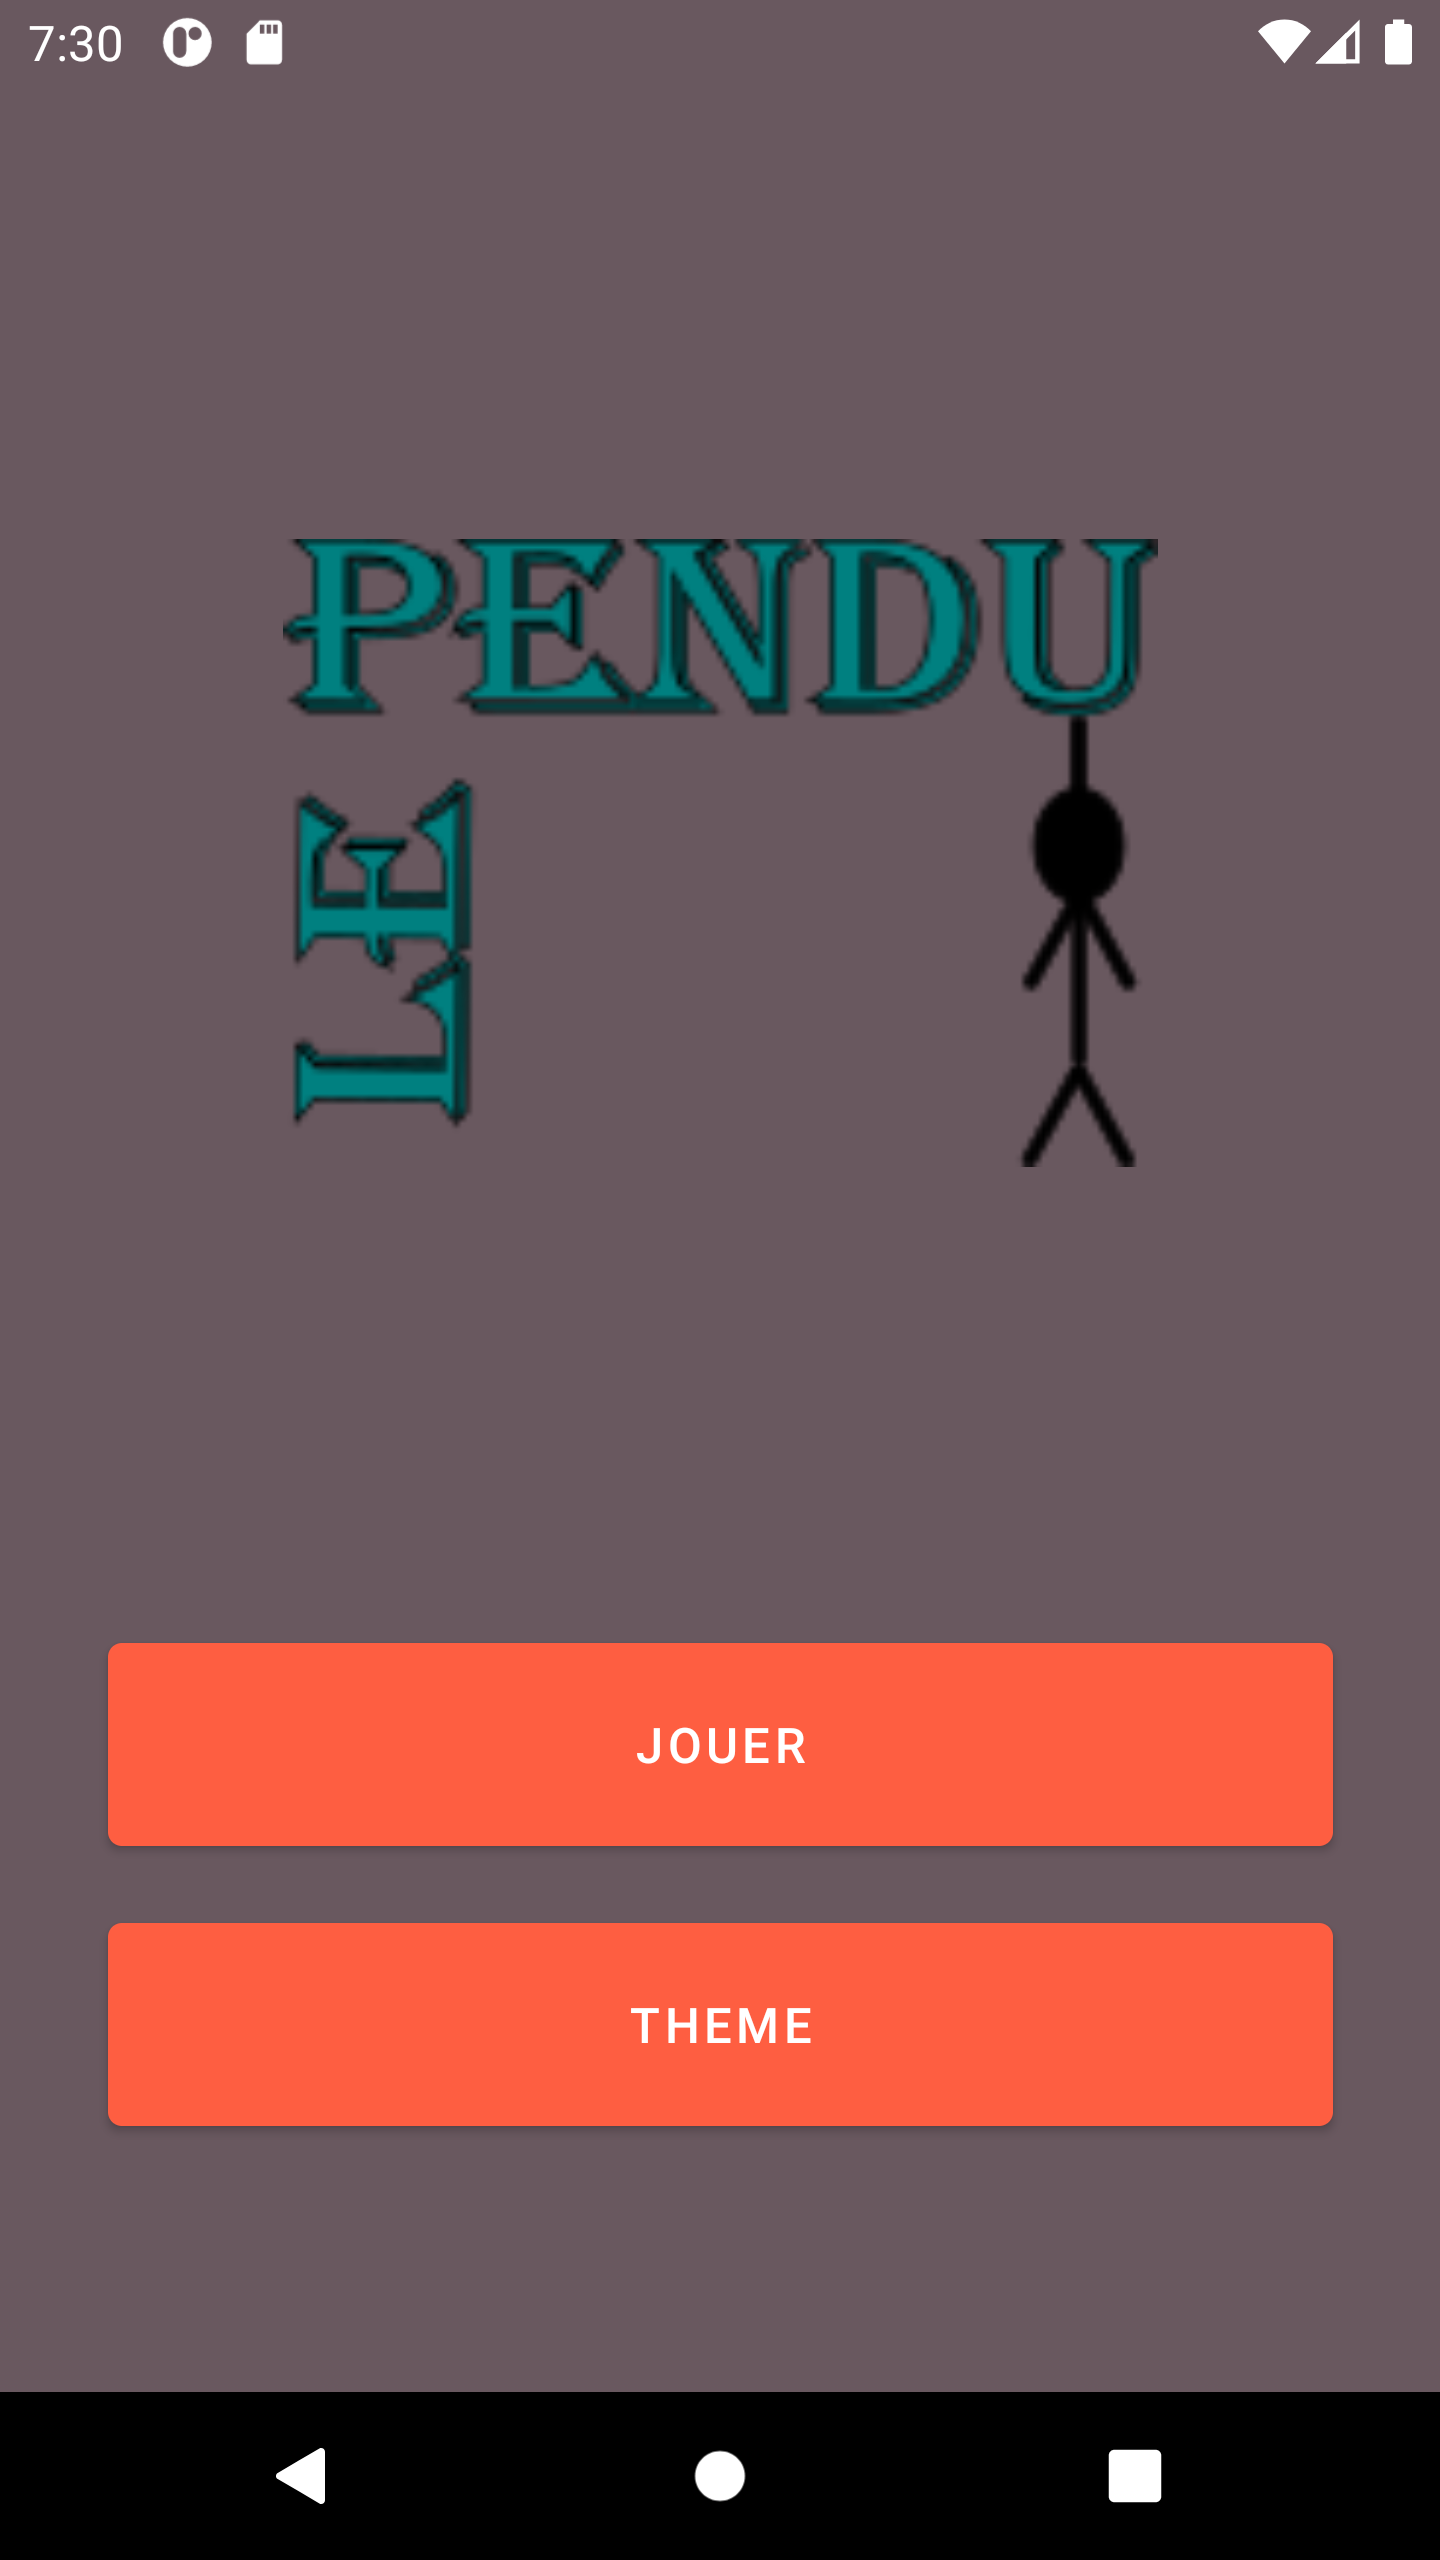
\includegraphics[scale=0.08]{menu.png}
\caption{Interface du menu }
\label{fig:menu}
\end{figure}
\newpage

Le Pendu génère aléatoirement des mots correspondant à un thème désignée. L'application possède huit thèmes différents. Elle est également composée d'un menu principale, d'un menu listant les huit thèmes, d'un menu permettant de jouer et de deux fenêtres pop-up permettant la gestion de la victoire.
\begin{figure}[!h]
    \centering
    \begin{subfigure}{}
        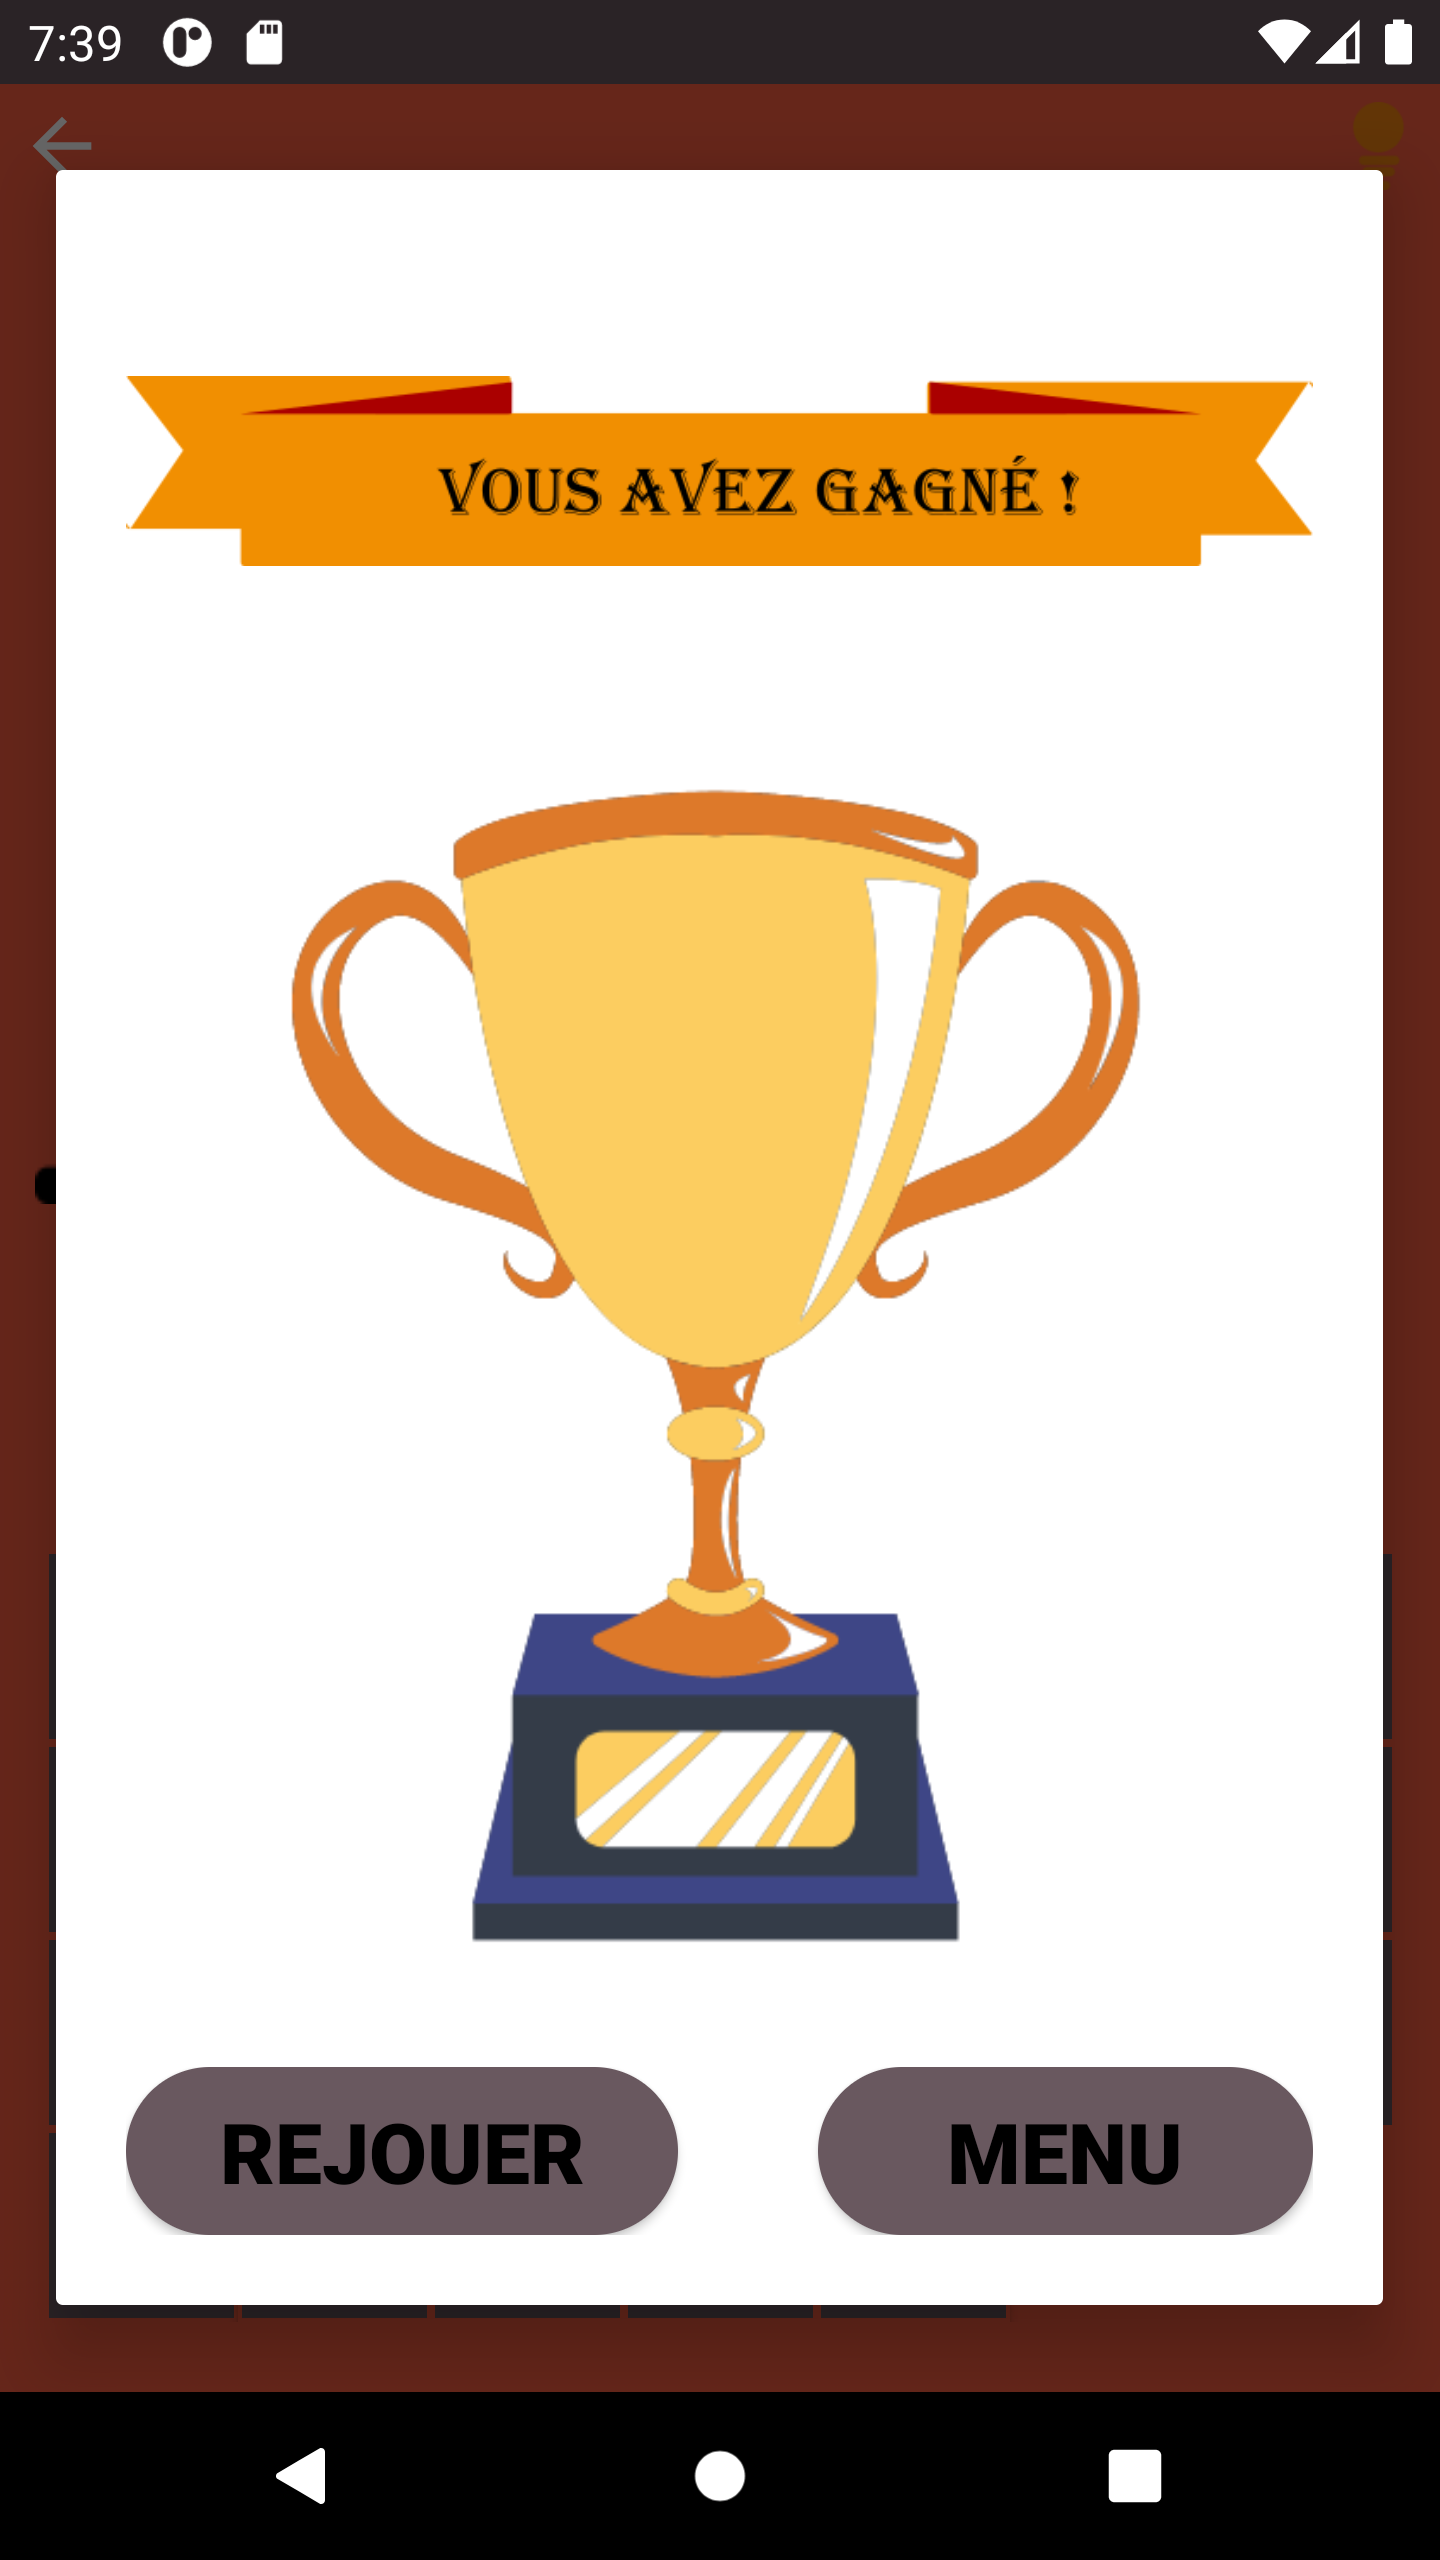
\includegraphics[scale=0.06]{victoire.png}
    \end{subfigure}
    \begin{subfigure}{}
        
\includegraphics[scale=0.06]{defaite.png}
    \end{subfigure}
    \caption{Pop-up de gestion de la victoire}
    \end{figure}
\\L'application sous Android possède plus de fonctionnalité que celle codé sur Xcode. En effet sous Android, un pop-up supplémentaire s'ajoute à ceux de la gestion de la victoire. Celui-ci correspond à un pop-up d'aide , permettant à l'utilisateur de voir une lettre ou d'obtenir un indice sur le mot en échange de pièce.





\begin{figure}[h!]
\color{black}
\centering

\includegraphics[scale=0.06]{aide.png}
\caption{Pop-up d'aide }
\label{fig:aide}
\end{figure}

À tout instant de l'application, l'utilisateur à la possibilité de revenir au menu et de changer de thème.

\newpage
\subsection{Design}
De nombreuses images illustrent le jeu du Pendu. Du logo, en passant par les illustrations de la liste, à l'état du pendu, tous ces éléments, on été réalisée sur le logiciel de dessin Inskape\cite{inskape}. Le choix des couleurs a été fait par l'usage d'une palette de couleur via le site Coolor
 \cite{colors}. 
\begin{figure}[h!]
\centering
\color{black}
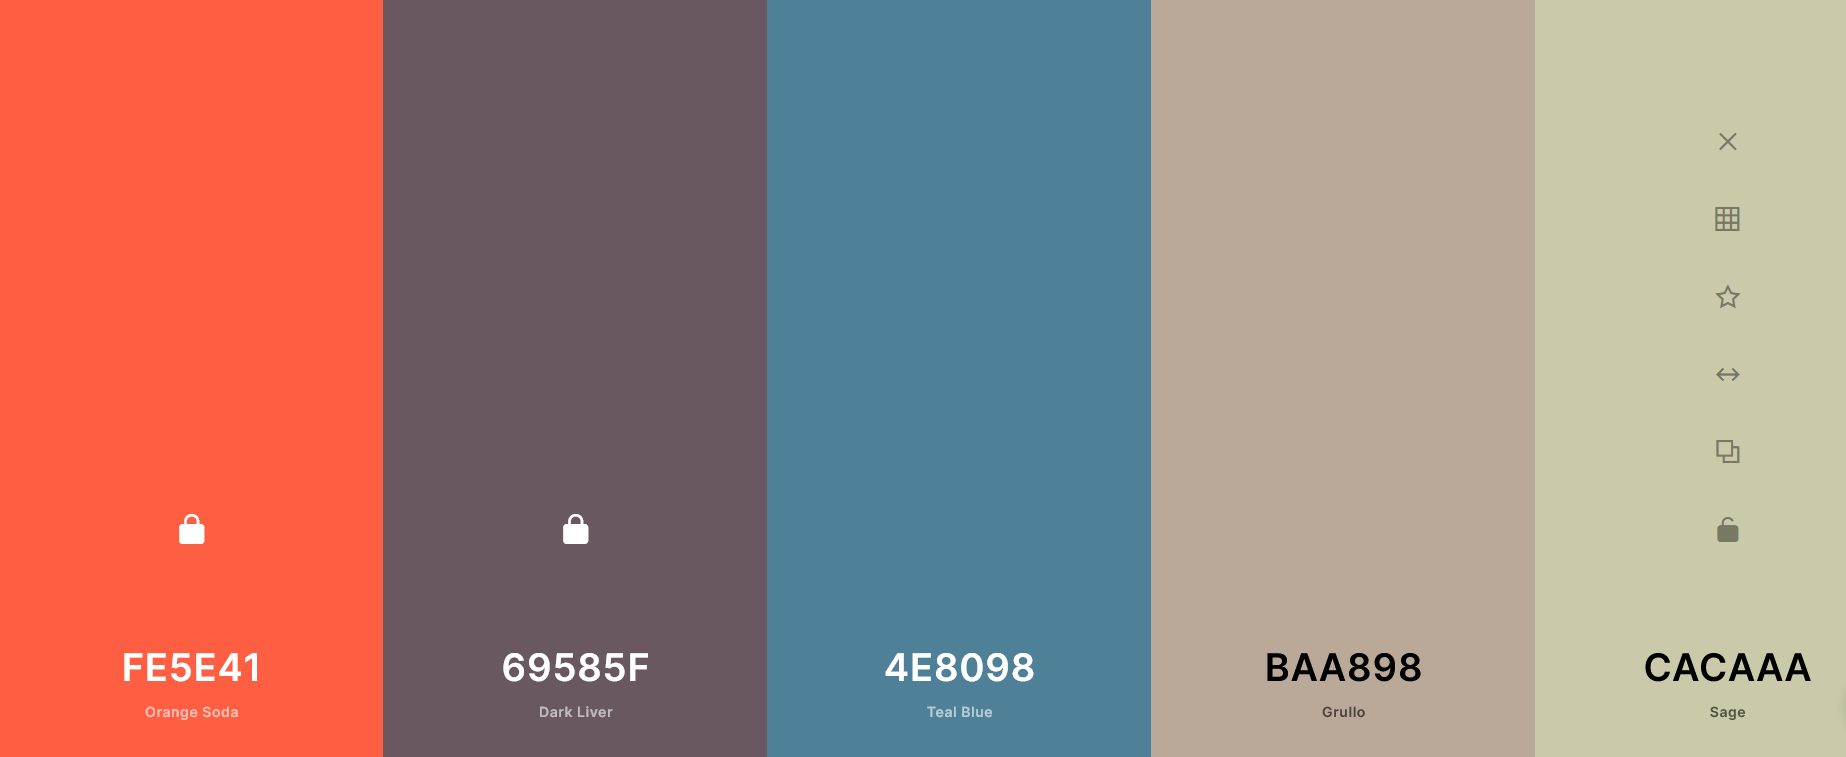
\includegraphics[scale=0.1]{Screenshot_2021-05-01 Create a palette - Coolors.png}
\caption{Palette de couleur de l'application }
\label{fig:couleur}
\end{figure}


\section{Interactions et Données au sein du jeu}
Le jeu comporte de nombreuses activités et pop-up qui communiquent entre eux. La communication dans l'application est illustrée ci-dessous.


\begin{figure}[h!]
\color{black}
\centering
\includegraphics[scale=0.2]{Légende_1_.png}
\caption{Communication dans l'application }
\label{fig:legende}
\end{figure}





\subsection{Android} %% une sous-section

La communication de données sous Android se fait via l'utilisation d'un Bundle. Dans l'application, selon le thème choisis par l'utilisateur, le menu jeu doit proposer une liste de mots en correspondance avec le thème. Voici quelques extraits de code illustrant la communication entre la liste et le jeu.

\vspace{10mm}

1 - Envoie de l'information vers le menu par la liste
\\
\\
\fbox{
\begin{minipage}{1\textwidth}
    
    \vspace{2mm}
    {\color{blue}Intent} i = {\color{blue} new} Intent(this,{\color{red} Activity\_\ menu.class}); \\
    i.putExtra("theme",{\color{red}"PAYS.txt"});\\
    startActivity(i);\\
   

     
\end{minipage}
}
\vspace{5mm}

2 - Réception de l'information par le menu
\\
\\
\fbox{
\begin{minipage}{1\textwidth}

   
   \vspace{2mm}
    {\color{blue}Bundle} word\_\ array; \\
    {\color{blue}protected void} onCreate({\color{blue}Bundle} savedInstanceState) \{\ \\
        super.onCreate(savedInstanceState); \\
        setContentView(R.layout.activity\_\ menu); \\
        word\_\ array = getIntent().getExtras();\\

       {\color{green} //On récupére le nom du fichier dans lequel se trouve les mots}\\
        {\color{blue}if} (word\_\ array != null) myArray = word\_\ array.getString("theme");\\
      
      \}\
\end{minipage}
}
\\
\\Sur la demande du menu jeu, les pop-ups de l'application se lancent, que ce soit via une fonction ou par l'intermédiaire d'un bouton.

\\
\\3 - Lancement du pop-up de gestion de victoire par la demande du menu jeu
\\

\fbox{
\begin{minipage}{1\textwidth}
   
    \vspace{2mm}
  {\color{blue} private void} closeWinDialog({\color{blue}Boolean} win)  \{\
      
       {\color{blue} Intent }j = {\color{blue}new} Intent(this, {\color{red}Activity\_\ menu.class});\\

       {\color{blue} if} (win ) dialog\_\ result.setContentView(R.layout.victoire);\\
       {\color{blue} else} \{\
        \\
            dialog\_\ result.setContentView(R.layout.defaite);\\
            {\color{blue}TextView} mot = dialog\_\ result.findViewById(R.id.textView4);\\
            mot.setText("Le mot à deviner était "+  word); \\ 
        \}\
        dialog\_\ result.show(); \\
   
\}\
     
\end{minipage}
}
\vspace{20mm}

\subsection{iOS} %% une autre sous-section
 Sous IOS, la transmission d'information se fait via des Segue. 
 \\
 1- Envoie de l'information vers le menu par la liste
  \\
   \\
 \fbox{
\begin{minipage}{1\textwidth}
    
    \vspace{2mm}
 {\color{blue}func tableView}(\_\ {\color{blue}tableView}: UITableView,{\color{blue} didSelectRowAt indexPath}: IndexPath)\{\ \\
        index = indexPath.row\\
       {\color{blue} performSegue}(withIdentifier: "theme", sender: nil)\\
          \}\
          \\
   {\color{blue} override func prepare}(for {\color{blue}segue}: UIStoryboardSegue, {\color{blue}sender}: Any?) \{\
           \\
          {\color{blue} if} segue.identifier == "theme" \{\ 
          
                \\let VCDestination = segue.destination as! {\color{red}MenuViewController} \\
                   VCDestination.theme = index \\
           \}\
          
          \}\
\end{minipage}
}
\\
\\
2 - Réception de l'information par le menu
\\


\fbox{
\begin{minipage}{1\textwidth}
     
    \vspace{2mm}
   {\color{blue} class MenuViewController}: UIViewController \{\
   \\ var theme = 0
    
\\
   {\color{blue} override func viewDidLoad() }\{\
      \\  super.viewDidLoad()

       
    \}\ \\
   {\color{blue} override func prepare}(for {\color{blue}segue}: UIStoryboardSegue, {\color{blue}sender}: Any?) \{\
    
   {\color{blue} if }segue.identifier == "jouer"\{\
         \\let VCDestination = segue.destination as! {\color{red}ViewController}
           \\  VCDestination.Theme = theme \}\ \}\
    

 {\color{blue}   @IBAction func infoTheme(_ sender: UIButton)} \{\
       \\ {\color{blue} performSegue}(withIdentifier: "jouer", sender: nil)
        
    \}\ \}\
    

 
\end{minipage}
}

\section{Amélioration}
L'application demandée devait être conçue dans un délai imparti, c'est pourquoi certaines parties du jeu nécessitent encore des améliorations.
Pour commencer, l'implémentation d'une base de données, pour amoindrir le nombre d'éléments dans le jeu et facilité la lisibilité du code. Une fonctionnalité de changement de langue a aussi été prévue, mais n'a pas eu le temps de voir le jour. Et enfin la mise en œuvre de différents niveaux, comme par exemple un niveau chronométré ou un niveau en anglais pour tester sa culture linguistique.
De même, une amélioration des contraintes sur les objets de l'application, et la création de la version paysage de l'application sur Xcode.

\section{Conclusion}
En conclusion, le développement de cette application a été pour moi très enrichissant. Je suis satisfaite de ce que j'ai pu accomplir sur les deux plateformes même si des améliorations peuvent être apportées.  
\newpage

%%% La bibliographie:
\bibliographystyle{plain}
\bibliography{references}

\end{document}
